\documentclass[tikz, rgb,dvipsnames]{standalone}
\usepackage{pgfplots}
\usepackage{xcolor}
\pgfplotsset{compat=newest}
\usetikzlibrary{calc,math}
\usetikzlibrary{shapes.misc}
\usetikzlibrary {arrows.meta}

\tikzset{>=latex}
\def\ColrGridLinesBackground{gray}
\def\ColrGridLinesFrame{black}
\def\Col{OliveGreen!15!white!75}

\def\ColA{red}
\def\ColB{red}
\def\ColC{red}
\def\W{4.8}
\def\H{3.6}

\def\hexsidelength{1}
\def\C{0.8660254037844386}
\def\hexhalfheight{\C * \hexsidelength}


\def\X{0.5 * \hexsidelength}
\def\Y{\hexhalfheight}

\newcommand{\GHexagonPlain}[3]{
\fill [color=#3]
(-\X + #1, -\Y + #2) --
( \X + #1, -\Y + #2) --
( \hexsidelength + #1, 0 + #2) --
( \X + #1,  \Y + #2) --
(-\X + #1,  \Y + #2) --
(-\hexsidelength + #1, 0 + #2) -- cycle;

% background divisions
\draw [color=\ColrGridLinesBackground, ultra thin]
(-\hexsidelength+#1, 0+#2)--(\hexsidelength+#1,0+#2)
( \X + #1, -\Y + #2) -- (-\X + #1, \Y + #2)
(-\X + #1, -\Y + #2) -- ( \X + #1, \Y + #2);
% frame around hexagon
\draw [color=\ColrGridLinesFrame]
(-\X + #1, -\Y + #2) --
( \X + #1, -\Y + #2) --
( \hexsidelength + #1, 0 + #2) --
( \X + #1,  \Y + #2) --
(-\X + #1,  \Y + #2) --
(-\hexsidelength + #1, 0 + #2) -- cycle;
}

\newcommand{\Hexagon}[3]{
    \GHexagonPlain{3*\hexsidelength*#1 + #2 * 1.5 * \hexsidelength}{#2 * \hexhalfheight / \hexsidelength}{#3}
}

\newcommand{\Dot}[3] {
    \fill[color=#3] (3*\hexsidelength*#1 + #2 * 1.5 * \hexsidelength
    , #2 * \hexhalfheight / \hexsidelength) circle (0.075);
}

\newcommand{\Label}[4] {
    \node at (3*\hexsidelength*#1 + #2 * 1.5 * \hexsidelength
    , #2 * \hexhalfheight / \hexsidelength) [#3] {#4};
}

\begin{document}
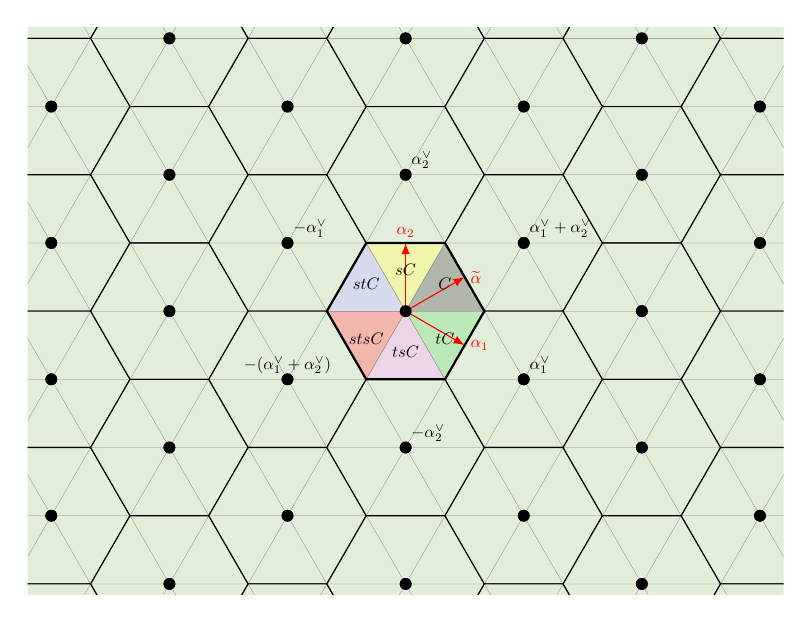
\begin{tikzpicture}[every node/.style={scale=0.6}]
    \clip (-\W, -\H) rectangle (\W, \H);
\foreach \x in {-5, ..., 5} {
\foreach \y in {-5,...,5} {
    \Hexagon{\x}{\y}{\Col}
    \Dot{\x}{\y}{black}
}
}

\coordinate (O) at (0,0);
\coordinate (A) at (\hexsidelength, 0);
\coordinate (B) at (\X, \Y);
\coordinate (C) at (-\X, \Y);
\coordinate (D) at (-\hexsidelength, 0);
\coordinate (E) at (-\X, -\Y);
\coordinate (F) at (\X, -\Y);

\fill[gray, opacity=0.5] (O) -- (A) -- (B) -- cycle;
\fill[Yellow!50, opacity=0.5] (O) -- (B) -- (C) -- cycle;
\fill[Blue!70!white!30!, opacity=0.5] (O) -- (C) -- (D) -- cycle;
\fill[Red!50, opacity=0.5] (O) -- (D) -- (E) -- cycle;
\fill[Violet!50, opacity=0.5] (O) -- (E) -- (F) -- cycle;
\fill[LimeGreen!50, opacity=0.5] (O) -- (F) -- (A) -- cycle;

% background divisions
\draw [color=\ColrGridLinesBackground, ultra thin]
(-\hexsidelength, 0)--(\hexsidelength,0)
( \X, -\Y) -- (-\X, \Y)
(-\X, -\Y) -- ( \X, \Y);
% frame around hexagon
\draw [color=\ColrGridLinesFrame, thick]
(-\X, -\Y) --
( \X, -\Y) --
( \hexsidelength, 0) --
( \X,  \Y) --
(-\X,  \Y) --
(-\hexsidelength, 0) -- cycle;

\draw[->, \ColA]
(0, 0) -- (0, \hexhalfheight) node[above] {$\alpha_2$};

\draw[->, \ColB]
(0, 0) -- (\hexhalfheight * \C, -\hexhalfheight * 0.5) node[below, right] {$\alpha_1$};

\draw[->, \ColC]
(0, 0) -- (\C*\C, \C*0.5) node[above, right] {$\widetilde{\alpha}$};




\foreach \x in {-5, ..., 5}
\foreach \y in {-5,...,5} {
    \Dot{\x}{\y}{black}
}



\coordinate (G) at (\X, \Y * 0.4);
\node at (G) {$C$};

\coordinate (H) at (0, \Y * 0.6);
\node at (H) {$sC$};

\coordinate (I) at (\X, -\Y * 0.4);
\node at (I) {$tC$};

\coordinate (J) at (-\X, \Y * 0.4);
\node at (J) {$stC$};

\coordinate (K) at (0, -\Y * 0.6);
\node at (K) {$tsC$};

\coordinate (L) at (-\X, -\Y * 0.4);
\node at (L) {$stsC$};

\Label{1}{-1}{above right}{$\alpha_1^\vee$}
\Label{-1}{2}{above right}{$\alpha_2^\vee$}
\Label{0}{1}{above right}{$\alpha_1^\vee+\alpha_2^\vee$}
\Label{-1}{1}{above right}{$-\alpha_1^\vee$}
\Label{0}{-1}{above}{$-(\alpha_1^\vee+\alpha_2^\vee)$}
\Label{1}{-2}{above right}{$-\alpha_2^\vee$}
\end{tikzpicture}
\end{document}
